\documentclass[12pt]{article}
\usepackage[utf8]{inputenc}
\usepackage{graphicx}
\usepackage{setspace}
\usepackage{hyperref}
\usepackage{biblatex}
\renewcommand{\contentsname}{Sisukord}
\setstretch{1.5}
\usepackage{geometry}
\usepackage[svgnames]{xcolor}
  \definecolor{diffstart}{named}{Grey}
  \definecolor{diffincl}{named}{Green}
  \definecolor{diffrem}{named}{OrangeRed}

\usepackage{listings}
  \lstdefinelanguage{diff}{
    basicstyle=\ttfamily\tiny,
    morecomment=[f][\color{diffstart}]{@@},
    morecomment=[f][\color{diffincl}]{+},
    morecomment=[f][\color{diffrem}]{-},
    backgroundcolor = \color{lightgray},
  }

\geometry{a4paper, portrait, margin=30mm, bmargin=30mm, tmargin=30mm}
\begin{document}
\begin{center}
\thispagestyle{empty}
\large{Tartu Ülikool}\\[-0.9ex]
\large{Loodus- ja täppisteaduste valdkond}\\
\large{Arvutiteaduse instituut}\\
\vspace{6cm}
\large{Joosep Näks}\\
\textbf{\LARGE{CVE-2020-4049}}\\
Referaat
\end{center}
\vspace{1.5cm}
\begin{flushright}
LTAT.06.002 Andmeturve\\
Õppejõud: Meelis Roos
\end{flushright}
\vspace{6cm}
\begin{center}
2021
\end{center}
\pagebreak

\tableofcontents

\pagebreak

\section{Sissejuhatus}

WordPress on vabavaraline blogihaldamise keskkond, kus saab blogi illustreerimiseks ka üles laadida blogi teemasid, mis muudavad seda, kuidas blogi välja näeb. Turvaauk CVE-2020-4049 on haavatavus teema faili üleslaadimisel, mis laseb teema failinime sisse peita JavaScripti skripti.\textsuperscript{[\ref{nvd}]}

Käesolevaga luban Tartu Ülikoolil seda referaati avalikult eksponeerida kuni aastani 2026.
\section{Turvaaugu kirjeldus}
Turvaauk laseb kasutajal laadida üles teema fail, mille nimesse on peidetud JavaScripti kood, ning seda koodi jooksutatakse blogi teema valimise lehel administraatori õigustega. Turvaaugu risk on madal, kuna ka teema üleslaadimiseks on vaja administraatori õigusi.\textsuperscript{[\ref{meilid}]}
\section{Ohtlikkus}

Üks võimalus turvaaugu ära kasutamiseks oleks see, kui ründaja veenaks psüholoogilise ründe abil blogi administraatorit üles laadima ründaja poolt koostatud ohtliku nimega teema faili ning seejärel kui ükskõik milline blogi administraator avab teemade lehe, käivitub ründaja loodud skript. Selle oht on siiski väike, kuna terve ründaja skript peab olema faili nime sees ehk blogi administraatoril on lihtne märgata, et tegu on kahtlase teema failiga.
\pagebreak

\section{Parandus}
Turvaauk on parandatud alates WordPressi versioonist 5.4.2. Paranduseks tehtud muudatus on järgnev:\textsuperscript{[\ref{git}]}\\
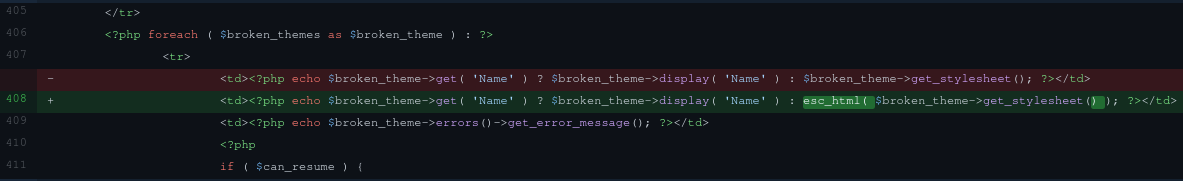
\includegraphics[scale=0.4]{andmeturve_pilt.png}\\
Teema faili sisselugemisse lisati funktsioon \texttt{esc\textunderscore html()}, mis leiab sisendist \texttt{HTML} sildid üles ning muudab nad selliseks, et \texttt{HTML} koodi parsimisel loetaks neid tavalise tekstina. \textsuperscript{[\ref{eschtml}]} See tähendab et teema faili nimes olevat skripti esitatakse tavatekstine ning see ei käivitu enam blogi teemade lehe avamisel.
\renewcommand{\refname}{Viited}
\begin{thebibliography}{9}
\bibitem{nvd}
\label{nvd}
\small{\url{https://nvd.nist.gov/vuln/detail/CVE-2020-4049#vulnCurrentDescriptionTitle}}
\bibitem{meilid}
\label{meilid}
Turvaaugu meililist:\\
\small{\url{https://lists.debian.org/debian-lts-announce/2020/07/msg00000.html}}
\bibitem{github}
\label{git}
Parandus githubis:\\
\small{\url{https://github.com/WordPress/wordpress-develop/commit/404f397b4012fd9d382e55bf7d206c1317f01148}}
\bibitem{eschtml}
\label{eschtml}
\small{\url{https://developer.wordpress.org/reference/functions/esc_html/}}
\end{thebibliography}
\end{document}